\documentclass{article}
\usepackage{amsmath}
\usepackage{booktabs}
\usepackage{geometry}
\usepackage{tikz}
\usepackage{pgfplots}
\pgfplotsset{compat=1.17}
\geometry{margin=1in}
\title{Fixed Income Trading Language Cheat Sheet}
\begin{document}
\maketitle

\section{Abbreviations}
\begin{itemize}
    \item \textbf{UB} = Ultra Bond (long-dated government bond).
    \item \textbf{RX} = Euro Bund (German government bond).
    \item \textbf{German Bond Futures}: Bund (8.5-10.5y), Bobl (4.5-5.5y), Shatz(1.75-2.25y)
    \item \textbf{UST}: Bonds (more than 10y), Notes (2y-10y), Bills (less than 1y - ZBC, issued at discount)
    \item \textbf{30s50s}: 50-year bond minus 30-year bond yield spread. 
\end{itemize}

\section{Price Movements}

\begin{itemize}
  \item Price $\uparrow$ $\Rightarrow$ Yield $\downarrow$ (called a \emph{rally}); Price $\downarrow$ $\Rightarrow$ Yield $\uparrow$ (a \emph{sell-off}).
  \item Cheapening = Price $\downarrow$ $\Rightarrow$ Yield $\uparrow$.
  \item Richening = Price $\uparrow$ $\Rightarrow$ Yield $\downarrow$.
  \item Market paid = Yield $\uparrow$ $\Rightarrow$ Price $\downarrow$.
\end{itemize}

\section{Long vs Short}

\subsection{Bonds}
\begin{itemize}
  \item \textbf{Long bond} = Receive fixed payments $\Rightarrow$ Position benefits if rates fall (bond prices rise).
  \item \textbf{Short bond} = Pay fixed $\Rightarrow$ Position benefits if rates rise (bond prices fall).
\end{itemize}

\subsection{Swaps}
\begin{itemize}
  \item \textbf{Buy a swap} = Pay fixed $\leftrightarrow$ Short bond-like exposure, receive floating. \textbf{Positive rate delta}.
  \item \textbf{Sell a swap} = Receive fixed $\leftrightarrow$ Long bond-like exposure, pay floating. \textbf{Negative rate delta}.
\end{itemize}

\noindent
In trader shorthand:
\[
\text{``Mine'' (in swaps)} = \text{Pay fixed},\quad
\text{``Yours''} = \text{Receive fixed}
\]

A tenor is cheap then we should try to receive fixed in that tenor, and if it is rich then we should pay fixed.

\subsection{Swap Spread}
The \textbf{swap spread} is defined as:
\[
\text{Swap Spread} = \text{Swap Rate} - \text{Government Bond Yield (same maturity)}
\]

\begin{itemize}
  \item Measures the risk premium of swap rates over risk-free Treasuries.
  \item A widening swap spread (↑) implies swap rates are rising relative to govies:
    \begin{itemize}
      \item Could reflect increased credit/liquidity risk in the swap market.
      \item Bullish for bonds (e.g., flight to quality).
    \end{itemize}
  \item A tightening swap spread (↓):
    \begin{itemize}
      \item Common during QE or balance sheet expansion.
    \end{itemize}
  \item \textbf{Long swap spread} = Receive fixed in swap and short the government bond.
  \item \textbf{Short swap spread} = Pay fixed in swap and long the government bond.
\end{itemize}


\section{Trade Language: Execution Slang}
\begin{center}
\begin{tabular}{@{}ll@{}}
\toprule
\textbf{Phrase} & \textbf{Meaning} \\
\midrule
“Hit my bid” / “I got hit” & I bought (someone sold to me) \\
“Lift my offer” / “I got lifted” & I sold (someone bought from me) \\
“Mine” & I buy \\
“Yours” & I sell \\
“Take” & I buy \\
“Give” & I sell \\
\bottomrule
\end{tabular}
\end{center}


\section{Yield Curve and Duration}

Movements in the yield curve provide insight into both rate direction and relative duration risk. Traders describe shifts using intuitive terms that bundle curve shape with rate momentum.

\subsection*{Types of Curve Shifts}

\begin{itemize}
  \item \textbf{Bull Steepener:}
    \begin{itemize}
      \item Short-end yields fall more than the long-end.
      \item Indicates easing expectations (e.g. central bank cuts).
      \item Duration shortens — gain more from front-end rally.
    \end{itemize}
  
  \item \textbf{Bear Flattener:}
    \begin{itemize}
      \item Long-end yields rise more than the short-end.
      \item Often due to inflation or supply fears.
      \item Duration lengthens — curve flattens with losses concentrated in the long end.
    \end{itemize}
  
  \item \textbf{Bull Flattener:}
    \begin{itemize}
      \item Long-end rallies more than short-end.
      \item Often a flight-to-quality move.
      \item Long exposure benefits more.
    \end{itemize}
  
  \item \textbf{Bear Steepener:}
    \begin{itemize}
      \item Short-end sells off more than long-end.
      \item Driven by hawkish monetary policy.
      \item Long exposure loses more quickly in the front end.
    \end{itemize}
\end{itemize}

\subsection*{Trader Mnemonic}
\begin{itemize}
  \item \textbf{S}teepening $\Rightarrow$ \textbf{S}horter duration exposure benefits
  \item \textbf{F}lattening $\Rightarrow$ \textbf{F}atter (longer) duration exposure benefits
\end{itemize}

\begin{figure}[h]
\centering
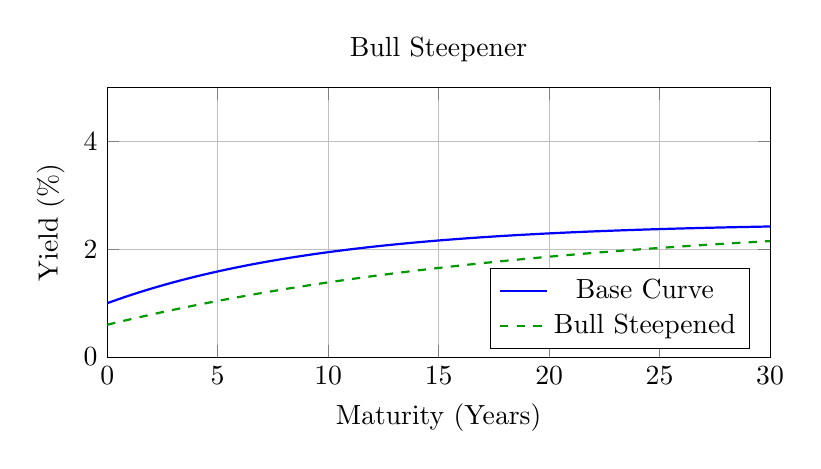
\begin{tikzpicture}
\begin{axis}[
    width=10cm, height=5cm,
    xlabel={Maturity (Years)},
    ylabel={Yield (\%)},
    xmin=0, xmax=30,
    ymin=0, ymax=5,
    legend pos=south east,
    title={Bull Steepener},
    grid=both,
    samples=100,
    domain=0:30
]
\addplot[blue, thick] {1.0 + 1.5*(1 - exp(-x/10))};
\addlegendentry{Base Curve}
\addplot[green!60!black, dashed, thick] {0.6 + 2.0*(1 - exp(-x/20))};
\addlegendentry{Bull Steepened}
\end{axis}
\end{tikzpicture}
\caption{Front-end rates rally more than long-end (short yields drop faster).}
\end{figure}

\begin{figure}[h]
\centering
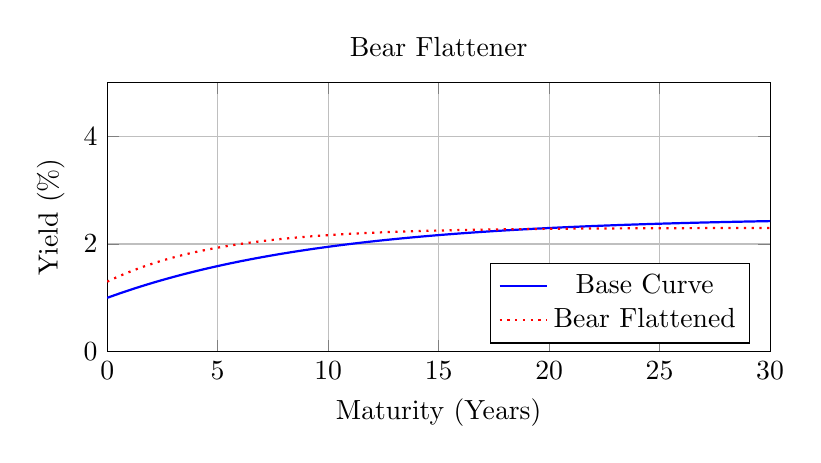
\begin{tikzpicture}
\begin{axis}[
    width=10cm, height=5cm,
    xlabel={Maturity (Years)},
    ylabel={Yield (\%)},
    xmin=0, xmax=30,
    ymin=0, ymax=5,
    legend pos=south east,
    title={Bear Flattener},
    grid=both,
    samples=100,
    domain=0:30
]
\addplot[blue, thick] {1.0 + 1.5*(1 - exp(-x/10))};
\addlegendentry{Base Curve}
\addplot[red, dotted, thick] {1.3 + 1.0*(1 - exp(-x/5))};
\addlegendentry{Bear Flattened}
\end{axis}
\end{tikzpicture}
\caption{Long-end rates rise more than short-end (flattening in bear market).}
\end{figure}

\begin{figure}[h]
\centering
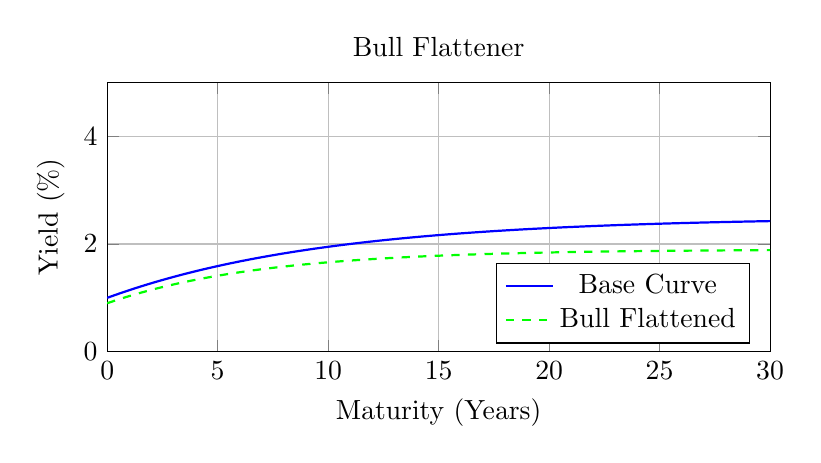
\begin{tikzpicture}
\begin{axis}[
    width=10cm, height=5cm,
    xlabel={Maturity (Years)},
    ylabel={Yield (\%)},
    xmin=0, xmax=30,
    ymin=0, ymax=5,
    legend pos=south east,
    title={Bull Flattener},
    grid=both,
    samples=100,
    domain=0:30
]
\addplot[blue, thick] {1.0 + 1.5*(1 - exp(-x/10))};
\addlegendentry{Base Curve}
\addplot[green, dashed, thick] {0.9 + 1.0*(1 - exp(-x/7))};
\addlegendentry{Bull Flattened}
\end{axis}
\end{tikzpicture}
\caption{Long-end rallies more than short-end (flight-to-quality move).}
\end{figure}

\begin{figure}[h]
\centering
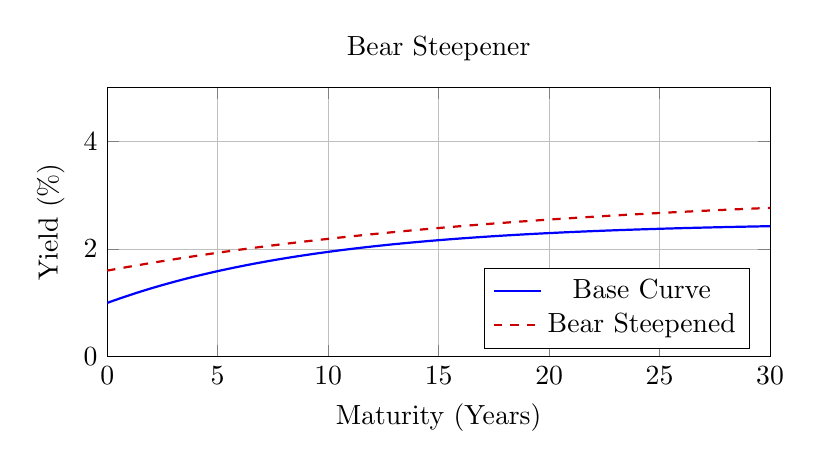
\begin{tikzpicture}
\begin{axis}[
    width=10cm, height=5cm,
    xlabel={Maturity (Years)},
    ylabel={Yield (\%)},
    xmin=0, xmax=30,
    ymin=0, ymax=5,
    legend pos=south east,
    title={Bear Steepener},
    grid=both,
    samples=100,
    domain=0:30
]
\addplot[blue, thick] {1.0 + 1.5*(1 - exp(-x/10))};
\addlegendentry{Base Curve}
\addplot[red!80!black, thick, dashed] {1.6 + 1.5*(1 - exp(-x/20))};
\addlegendentry{Bear Steepened}
\end{axis}
\end{tikzpicture}
\caption{Front-end sells off more than long-end (hawkish surprise).}
\end{figure}


\subsection*{Interpretation for Trading}
\begin{itemize}
  \item \textbf{Flatteners} benefit trades that are long duration (e.g. receive fixed on long swaps).
  \item \textbf{Steepeners} reward trades with more front-end exposure (e.g. pay fixed short, receive long).
  \item Relative value trades often structure exposure via curve slope rather than outright direction.
\end{itemize}


\end{document}
